%---------------------------------
% CHAPTER 3: Scope of the project
%---------------------------------

\chapter{Offer and demand comparison}

\label{chapter03}

Knowing the context inside \company\ and all the state of the art of this project, the definition and scope is well defined.

%-----------------
%   SECTION 3.1
%-----------------

\section{Formulation of the problem} \label{problem}

The main goal of this project is creating a tool for \textit{\company} to ease the routes comparison with different parameters, taking into account values like \textbf{user searches} and \textbf{flights available} by airlines.
\\\\
In any team of \company, user queries and providers data is compared in order to guess valuable trends.
\\\\
Found that gap, a bunch of new ideas appeared. After some talks with product owners of different squads and some senior engineers, a promising idea showed up:
\\\\
Comparison of \textbf{user searches} and \textbf{flights available} by airlines, enabling finding \textit{over-requested} routes or airports. Those routes or airports with more user demand than availability by the providers.
\\\\
\squad\ manages a huge amount of data: All flights planned for the next year and a half, these are more than 75 million records. The database of all user queries in the website or mobile application is even bigger, there are 4 million visitors per day and a total of 13 million queries per day. Not much more information needed to say that this is \textbf{Big Data} problem.
\\\\
With \squad's product owner help, we found some use cases for the processing of those 75 million routes and all user session's queries to get some significant results:
\\\\
Provide a \textbf{visual tool} to find routes with much \textbf{more demand than offer} and be able to observe the \textbf{evolution} of it {through time}:

\begin{itemize}
  \item A route with a lot of demand, but not enough offer to cover it, will be \textbf{over-requested}.
  \item A route with much more offer, but not that amount of demand, will be \textbf{non-profitable}.
\end{itemize}

%-----------------
%   SECTION 3.2
%-----------------

\section{Scope}

Merging both data sources (providers and users) generates a lot of new valuable data with a lot of different application: From simply selling it to providers, to complex deep learning systems.
\\
The final goal of this project is displaying the comparison in a simple Web UI for Marketing squads or tribes. This can be split in three smaller goals or components:

\subsection{Pipeline}

Distributed application that maps and merge all the data from both sources in its given format to the required data model.
\\\\
The pipeline reads from \nameref{mp_engine} and \nameref{data_tribe} services. Then, it maps the provider and user data to the desired data model. The new entities are stored in a database where the service will read from.
\\\\
The application will be split in two sub applications, one for providers data and other for users. So both of them can vary independently without depending on each others' sources and changes may have in the future.

\subsection{Service}

Simple HTTP Service with a basic Application Programming Interface to serve Pipeline's results. The service will have an internal endpoint only available for other \company\ applications or developers.

\subsection{Visual representation} \label{visual_representation}

Website with a visual representation of the data. There are plenty of ways to draw charts and maps visualizations. The Web UI will be composed by two pages:

\subsubsection{Browser} \label{browser}

Simple browser with four input text fields, one for the origin airport, the second for the destination and the last two for the date, month and year.
\\\\
Once the inputs are set, the user will be able to click the \textit{Search} button and move to the next page.

\subsubsection{Chart visualization} \label{chart_visualization}

Simple chart with the comparison between providers offer and user demand of the selected entity through time.

\begin{figure}[H]
\centering
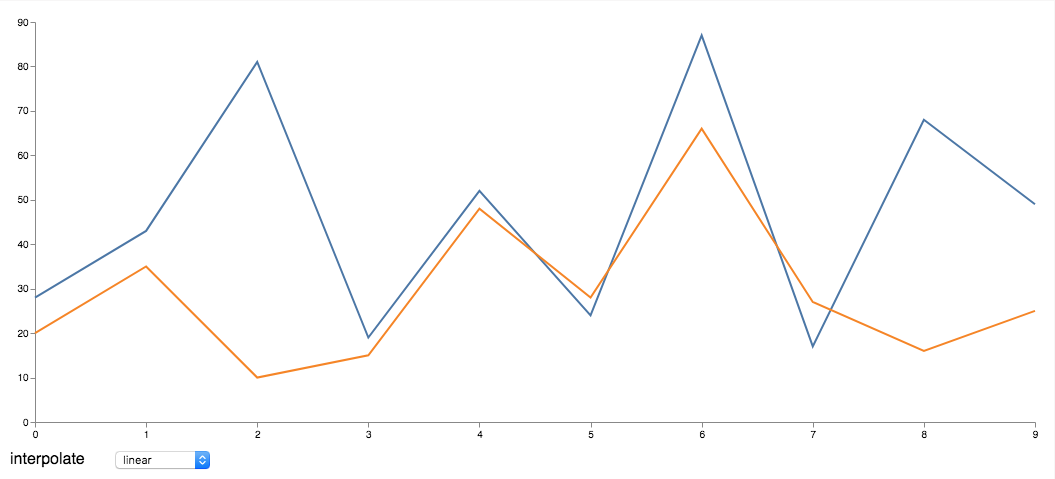
\includegraphics[scale=0.4]{resources/lineal-chart-example01.png}
\caption{Chart mock-up. One color goes for Providers Offer and the other one for User Demand.}
\end{figure}

\subsection{Not list} \label{not_list}

It is also important to define what this project will \textbf{not} be.

\begin{itemize}
  \item \textbf{Prices} or \textbf{quotes}: In any moment will check for flight prices or quotes.
  \item \textbf{Carriers}, \textbf{cities} and \textbf{countries}: The comparison will be only available between routes and airports, not airlines (carriers), cities nor countries.
  \item \textbf{Create}, \textbf{update} or \textbf{delete} data through the \textbf{Server}: The only input will come from the pipeline. Entities are never deleted or modified in order to keep historical data.
  \item \textbf{Create}, \textbf{update} or \textbf{delete} data through the \textbf{Web UI}: The only input will come from the pipeline. Entities are never deleted or modified in order to keep historical data.
\end{itemize}

%-----------------
%   SECTION 3.3
%-----------------

\section{Risks}

There are several risks can appear while developing the project. Most risks appear because of the dependencies with other tribes and squads and dependencies with other services. In the other hand, all performance risks of the Pipeline can be ignored because \company's hardware is enough for big applications, like this one.

\subsection{Routes contract}

\squad's routes service is under development and during the \thesis\ development the routes data model may change a little bit. For example, the origin and destination recently changed: In December 2017 the service was giving an \textit{Airport ID}, but now is giving an Airport object with more parameters like IATA Code\cite{iata_code}, Country ID, City ID, etc.

Timetables are served, basically, in three different models: Unified Routes, Single Flight Number Routes and Summary Routes. Both Single Flight Number and Summary Routes stores timetables by days of week\footnote{Explanation of different models in section \nameref{routes_model} on page \pageref{routes_model}}. The current \textbf{Unified Model} is supposed to be the final one, has been studied and refined by experts on the domain and \squad\ has been adapting the output until reaching this final model. Even so, it is impossible to guess if there will be some changes.

\subsection{Users information}

In the website and mobile application, the user have plenty of different ways to search the perfect flight. The most common one is by origin, destination and date, but he/she can also search by month or by destination. Then, the user is not searching flights by route and date. It sets the period of time he/she can travel and \company\ offers cheap destinations.
\\\\
Even searching by origin, destination and date, there can be invalid search queries. There are a lot of \textbf{cities with more than one airport} and usually when travelers search for traveling from there or to that city, they set the origin or destination \textbf{city}, but no the airport. For example: If you want to travel from New York to London, you have a lot of airports in New York (JFK, LGA, BUF, ROK, ALB, etc.), which provably only three will be useful for that search. And a total of six airports in London (LCY, LHR, LGW, LTN, STN, SEN). The final purchase, if there is, will be from two \textbf{airports}, but the \thesis\ looks for user intentions, not for final purchases.

\subsection{Amount of data}

As explained before in the \nameref{problem}, there is a very big amount of data that need to be mapped. Luckily, \company\ have great cloud machines and \textit{unlimited} space\footnote{Read more in section \nameref{resources}}. Anyway, still an issue to be aware of.
\\\\
The data processing will not be an actual issue, other teams already process the same amount or more data than the \thesis\ will do. This project's data source is already processed data from its original sources. \squad\ gets much more data from \nameref{sh_oag}, filters it, aggregates it with other inside company sources and writes the whole dump. Data tribe processes all user queries, flights, hotels and car hires.
\\\\
If in some point this became an issue I can ask for help to \squad\ members or data scientist.

\subsection{Kind of data}

User searches and flights offer have very similar parameters: origin, destination, date, etc. But can be very different. There are some facts that can give very different numbers for the same route and date, for example, seats in a plane. The flight offer pipeline counts number of flights, not of available seats. Is not the same one flight from Barcelona to Sydney that the aircraft will provably have 500 seats, than one flight Barcelona Mallorca that the aircraft will be much smaller and will barely reach 100 seats.

\subsection{Web UI}

Creating the interactive map and plots for the proposed website from zero, is a whole project itself. In order to avoid failing in the \textit{\nameref{visual_representation}} goal, the best option is to use reliable libraries, like Vega\cite{vega}. Combining it with React.js \company\ components, the Web UI development will be fast and easy.

%-----------------
%   SECTION 3.4
%-----------------

\section{Methodology and rigor} \label{methodology_rigor}

\subsection{Extreme Programming} \label{xp}

This project will be developed along with \squad's work. This squad is following Scrum, an agile methodology. After some research and discussions with the rest of the team, Extreme Programming (XP)\cite{xp} showed up as the best option.
\\\\
Extreme Programming is a style of software development focused in excellent applications, programming techniques and clear communication. To accomplish that, XP includes a philosophy of software development, body of practices, complementary principles and a community that shares these values.
\\\\
This methodology works with short development cycles, resulting in early, concrete and continuing feedback. Has an incremental approach, making way to a flexible schedule for the implementation. It relies in oral communication and tests to reach the goal of the project.

\begin{figure}[H]
\centering

\includegraphics[scale=0.25]{diagrams/extreme_programming.png}
\caption{Extreme programming planning loops.}
\end{figure}

The original Extreme Programming methodology is for teams of developers, but this project will be only developed by myself, so the original idea has been modified a little bit. The pair programming and pair negotiation has been removed because I have nobody to pair with. In order to have some feedback and update the requirements properly with the supervisor approval, I will be attending all \squad\ stand up meetings and explaining my progress and, if necessary, create meetings with the product owner and the rest of the squad to take the project on the right track.


\subsection{\texttt{git}}

GitLab will be the main tool for version control of the source code and issue tracking of different tasks. GitLab\cite{gitlab} is very similar than the well known Bitbucket\cite{bitbucket} and Github\cite{github}, all these tools are suitable for the development of the project, but \company\ uses only GitLab.
\\\\
All code projects (pipelines, service and website) will be stored in a project space in \company's GitLab domain called Heatmap\footnote{Heatmap was the original name of this project, the name remains the same since then}. Using \texttt{git}, the versions will be forked in branches. Branches allow fork code versions and then merge them all together in a master single branch with a better conflict control. Each branch will stand for an specific issue, \texttt{master} will be the main branch where the latest production version will be.

\begin{itemize}
    \item \textbf{\texttt{master}} branch will contain the accepted version of the project, this version must work in production with no error and must be tested in its development of task branch
    \item \textbf{Development branches} (named following the style \texttt{ISSUE\_NUMBER-ISSUE\_TITLE}) contains all development commits and code for a given task planned previously in the iteration plan. Those branches are tested in \nameref{sandbox} environment 
    \item \textbf{Bug fixing branches} (named \texttt{HOTFIX-BUG\_NAME}) are branches created for fixing bug in production. The idea is to apply a fast solution in the branch and merge it directly to \texttt{master}, so the bug is fixed as fast as possible, then create an issue to find a better solution with more time.
\end{itemize}

\subsection{Continuous delivery}

In order to deploy pipelines and services automatically when merging to \texttt{master}, the projects have integration with Drone\cite{drone}. Every time it commit to a branch, the application is build, tested and, if everything goes well, it deploys to \nameref{sandbox}. When merging to master, Drone automatically deploys to \nameref{prod}.

\subsection{Tasks and issues}

The \textbf{issue tracker} provided by GitLab\cite{gitlab} will be very helpful in order to monitor the evolution of the project. Issues will be composed by a title, description, milestone, labels (if needed), due date and weight, and represents a new functionality. In order to know the status, issues will be listed in three columns:

\begin{itemize}
    \item \textbf{Backlog:} Known tasks that haven been started yet. Could be a well defined task, with a very clear description, a due date and weight, or just a draft with empty fields.
    \item \textbf{WIP:} Work in Progress. The task is being considered, developed or tested.
    \item \textbf{Done:} Tasks finished, tested and working fine. Ready for merging into \texttt{master} and deploy to production.
\end{itemize}

\subsection{Environments}

In \company, for almost all Amazon Web Services resources, there are two different environments: Sandbox and Production, also known as \textit{prod}.

\subsubsection*{Sandbox} \label{sandbox}

In this environment, every developer is allowed to do whatever they want, they can create, edit and remove every resource, execute whatever program, query, etc. For this project, all resources but user demand data source is available in sandbox.
\\\\
Every three months, Cloud Operations squad cleans all Sandbox resources.

\subsubsection*{Prod} \label{prod}

In prod things work little different, first of all, in order to get a profile you need a project, without project you cannot create anything. Once you have the project's profile, it have no permission to do anything, this is different than Sandbox as well. In order to get permissions you have to raise a ticket to Cloud Operations squad.

